\documentclass[a4paper, 12pt, brazilian]{article}
\usepackage[T1]{fontenc}

\usepackage{amsmath, amsfonts, amssymb}
\usepackage{siunitx}

\usepackage[
top=2cm,
right=3cm,
bottom=2cm,
left=3cm
]{geometry}

\usepackage{xcolor}
\usepackage{tikz}
\usepackage{import}
\usepackage{float}

\usepackage{graphicx}
\usepackage{hyperref}
\usepackage{cleveref}
\usepackage{bm}
\usepackage{multirow}
\usepackage{cancel}
\usepackage[version=4]{mhchem}
\newcommand{\purple}[1]{\textcolor{magenta}{#1}}

\usepackage{config}

\begin{document}
	\section{Primeira questão}
	Calcule a energia fornecida pela bomba ($h_{b}$ em \SI{}{\meter}, com duas casas decimais) considerando o esquema abaixo. O aspersor localizado no ponto 2 opera com pressão de $\SI{4}{\kilogram f/\centi\meter^{2}}$ e a vazão que escoa na canalização é de $\SI{10}{\meter^{3}/\hour}$. O diâmetro da tubulação é de \SI{50}{\milli\meter} e a perda de carga total entre os pontos 1 e 2 é de \SI{15}{\meter}. A carga cinética no ponto 1 é desprezível e este ponto é uma superfície livre sujeita a pressão atmosférica. A cota em 1 vale \SI{100}{\meter} e em 2 vale \SI{146.3}{\meter}.
	\begin{center}
		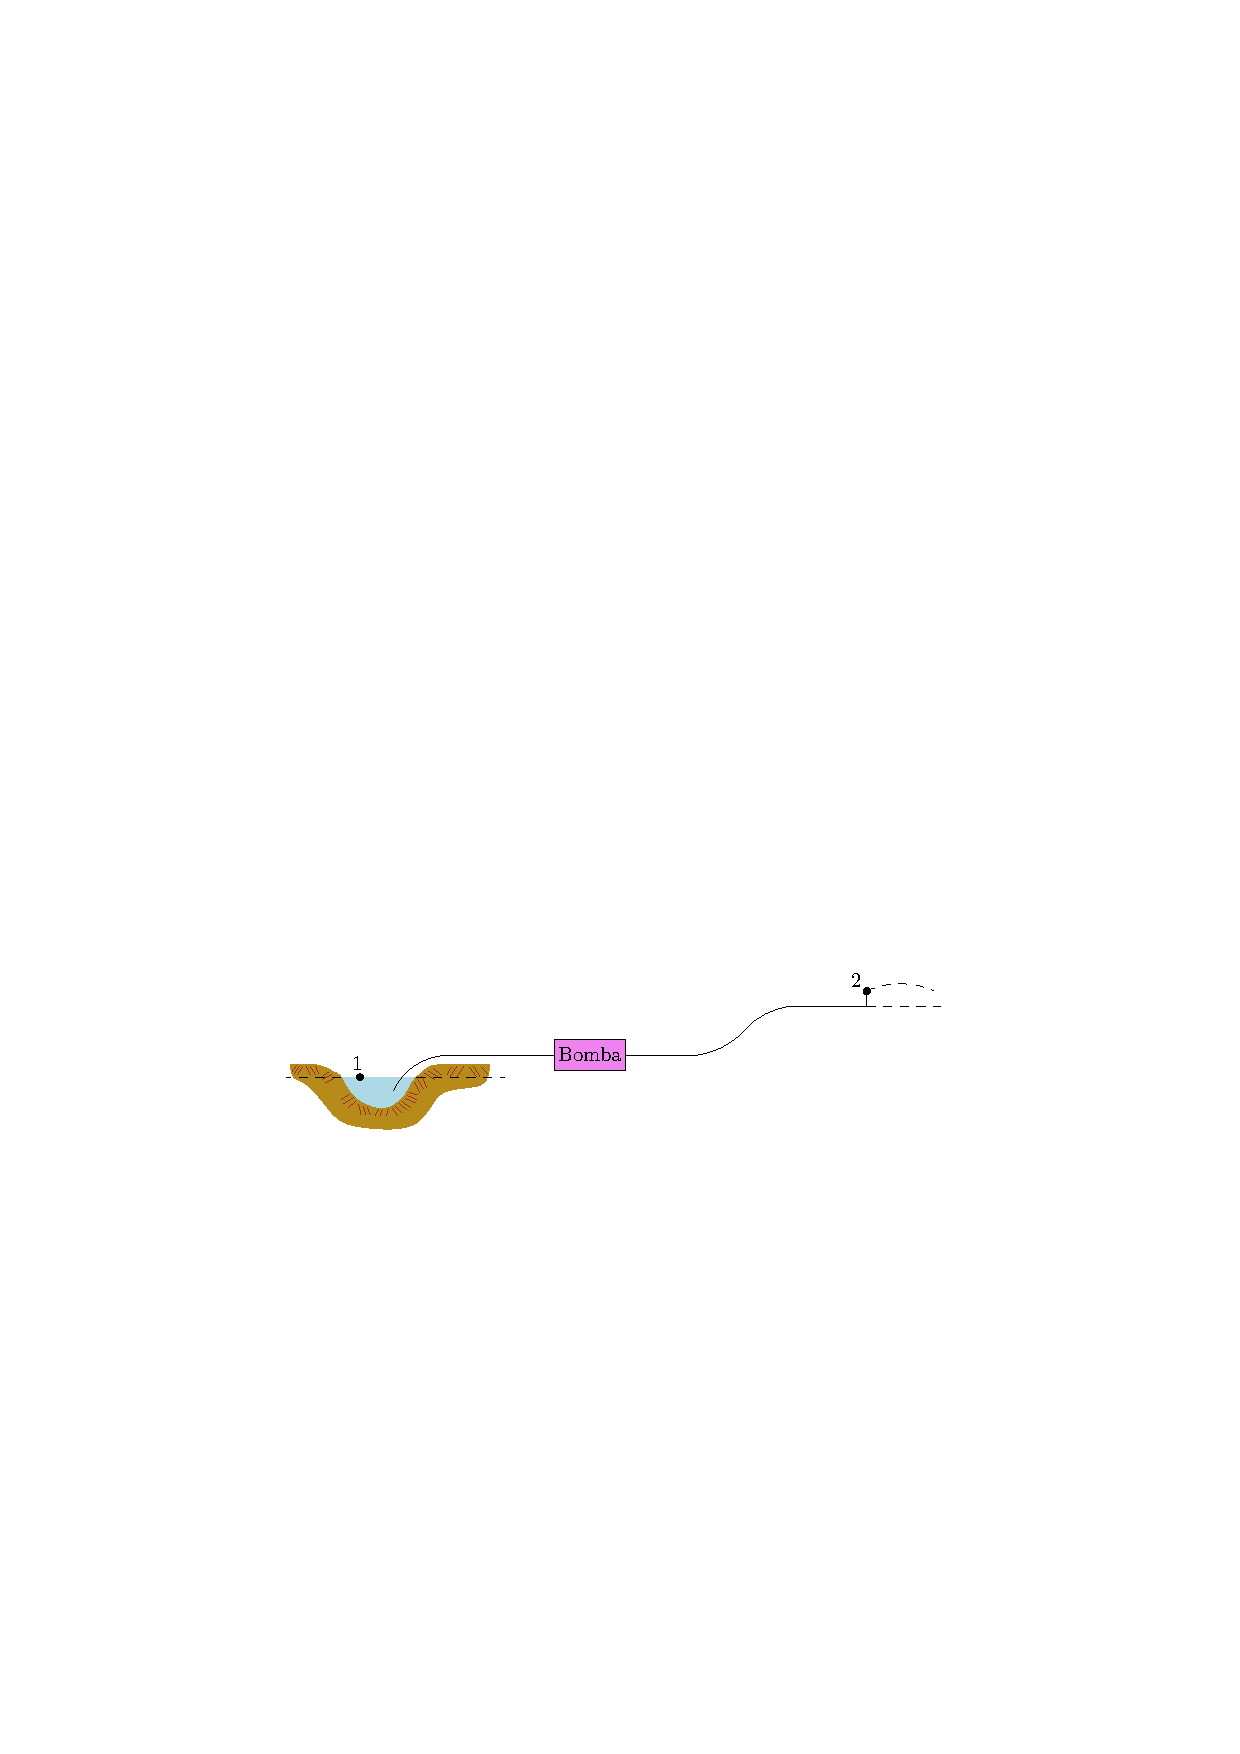
\includegraphics[width=.9\linewidth]{assets/images/ex1}
	\end{center}
	\subsection{Solução}
	A energia fornecida pela bomba pode ser dada pela equação de Bernoulli modificada como segue
	\begin{equation}
		\label{eq:bernoulli}
		Z_{1}+\dfrac{v_{1}^{2}}{2g}+\dfrac{p_{1}}{\gamma}+h_{b}=Z_{2}+\dfrac{v_{2}^{2}}{2g}+\dfrac{p_{2}}{\gamma}+hf_{1-2}
	\end{equation}
	A partir do que é dito no enunciado algumas simplificações podem ser feitas na equação anterior. Ao mudar o referencial das cotas é possível desprezar $Z_{1}$ fixando $Z_{2}=\SI{46.3}{\meter}$. No ponto 1 é cabível desprezar a pressão atuante, já que somente as moléculas da atmosfera agem. A carga cinética também é desprezada. Do lado direito da Equação de Bernoulli todos os termos serão considerados, só que para haver a substituição dos valores visando calcular $h_{b}$ as devidas conversões devem ser feitas para o Sistema Internacional.
	\begin{center}
		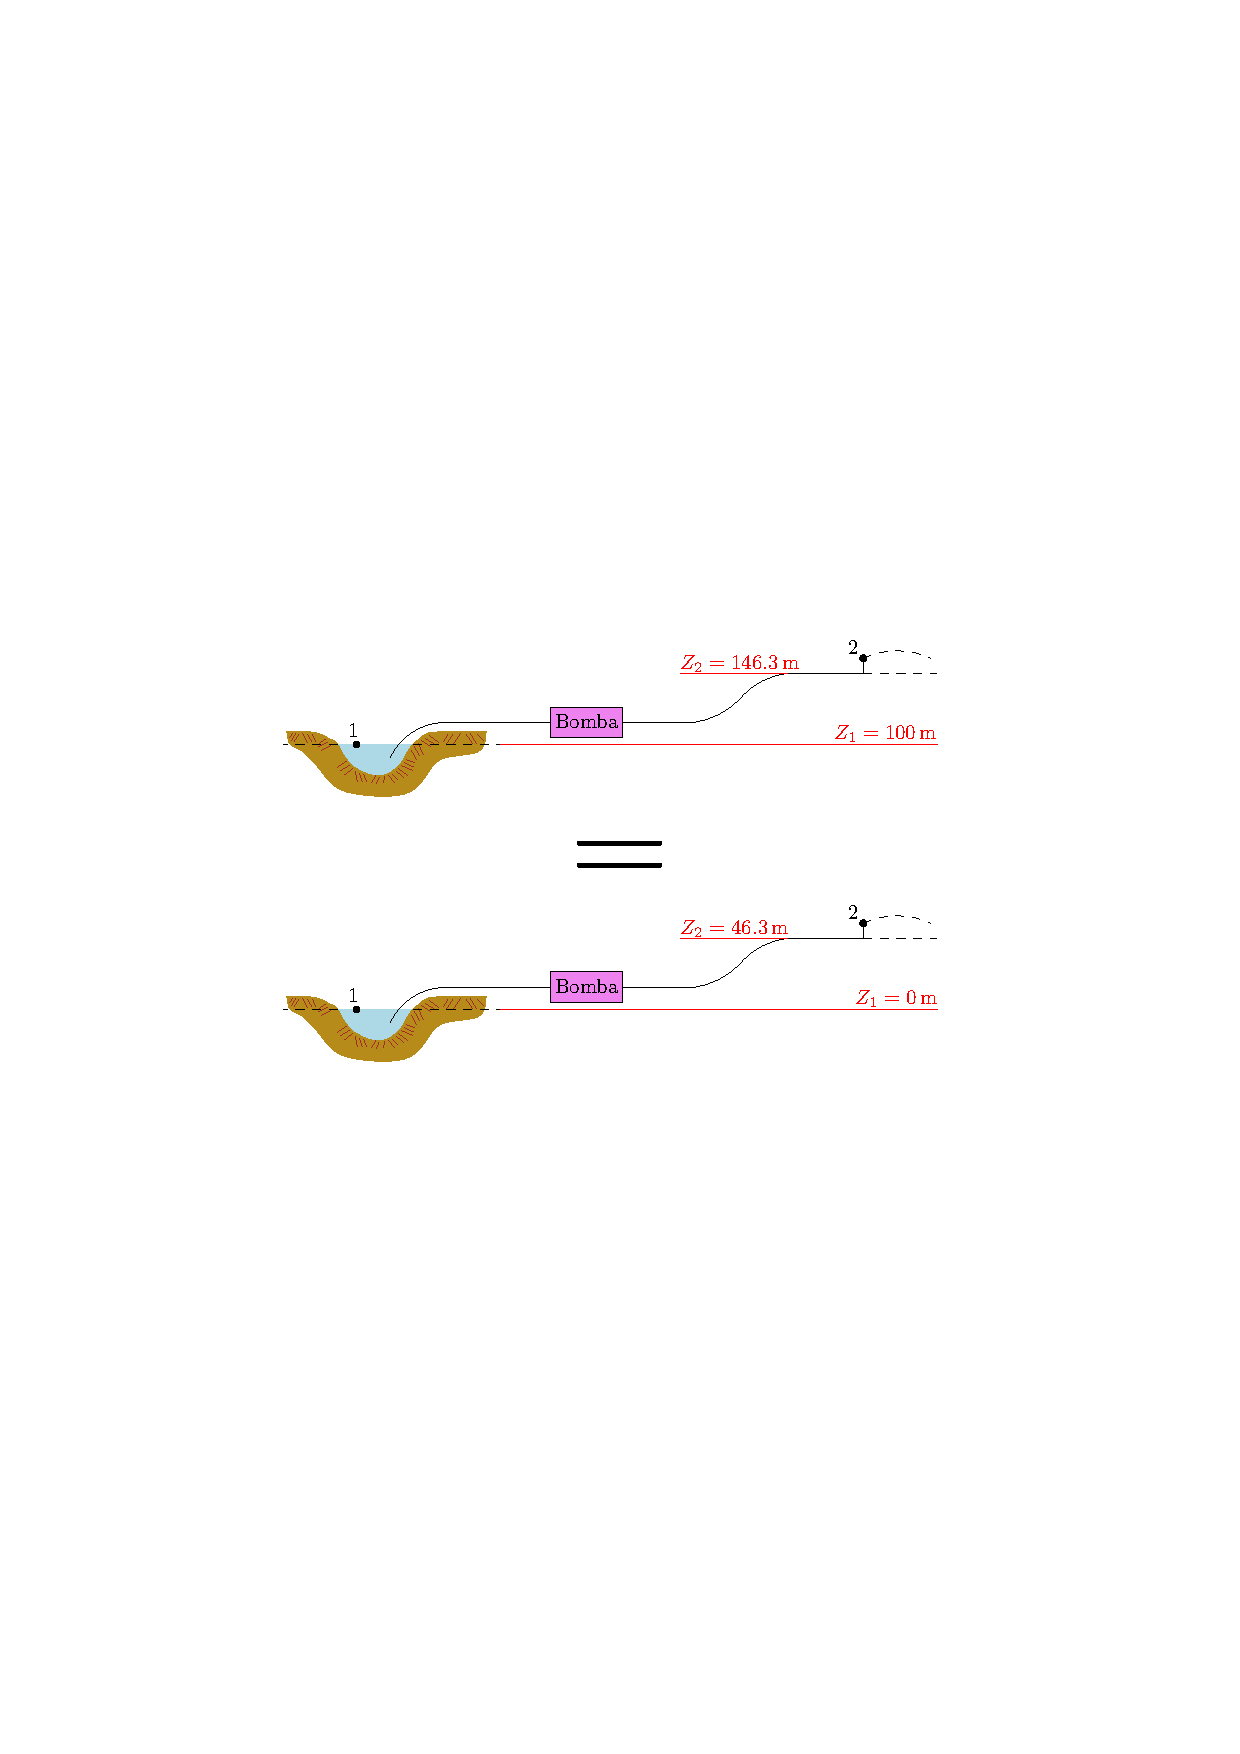
\includegraphics[width=.9\linewidth]{assets/images/referencia_1}
	\end{center}
	Para a pressão, é sabido que \SI{1}{\kilogram f} corresponde a \SI{9.81}{\newton}, então
	\begin{eqnarray}
		p_{2}&=&\SI{4}{\dfrac{\kilogram f}{\centi\meter^{2}}}\\
			 &=&\dfrac{4\cdot 9.81}{(10^{-2})^{2}}\SI{}{\dfrac{\newton}{\meter^{2}}}\\
			 &=&\SI{392400}{\pascal}
	\end{eqnarray}
	A vazão dada em $\SI{}{\meter^{3}/\hour}$ deve ser convertida para $\SI{}{\meter^{3}/\second}$ como segue
	\begin{eqnarray}
		Q_{2}&=&\SI{10}{\dfrac{\meter^{3}}{\hour}}\\
			 &=&\dfrac{10}{3600}\SI{}{\dfrac{\meter^{3}}{\second}}\\
			 &=&\SI{2.777e-3}{\meter^{3}/\second}
	\end{eqnarray}
	Após obter a vazão $Q_{2}$, para calcular a velocidade é preciso considerar a fluxo de água que atravessa a seção transversal do tubo como é descrito pela equação
	\begin{equation}
		Q_{2}=v_{2}\cdot A
	\end{equation}
	assim
	\begin{eqnarray}
		Q_{2}&=&v_{2}\cdot\dfrac{\pi d^{2}}{4}\Rightarrow\\
		\Rightarrow	v_{2}&=&\dfrac{4Q_{2}}{\pi d^{2}}
	\end{eqnarray}
	como $d_{2}=\SI{50}{\milli\meter}=\SI{.05}{\meter}$, vem
	\begin{eqnarray}
		v_{2}&=&\dfrac{4\cdot 0.00277}{\pi\cdot 0.05^{2}}\\
			 &=&\SI{1.411}{\meter/\second}
	\end{eqnarray}
	Substituindo em \eqref{eq:bernoulli}
	\begin{eqnarray}
		h_{b}&=&Z_{2}+\dfrac{v_{2}^{2}}{2g}+\dfrac{p_{2}}{\gamma}+hf_{1-2}\\
			 &=&46.3+\dfrac{1.411^{2}}{2\cdot 9.81}+\dfrac{392\,400}{9\,810}+15\\
			 &=&\purple{\SI{101.40}{\meter}}
	\end{eqnarray}
	\section{Segunda questão}
	Após percorrer o trecho vertical $AB$, a água descarrega em forma de jato na atmosfera, como mostra a figura abaixo. Sabendo que o diâmetro do tubo $A$ é quatro vezes maior que o de $B$ e que a pressão no ponto $A$ é de $\SI{.58}{\kilogram f/\centi\meter^{2}}$, estime a altura $H$ do jato (resultado em \SI{}{\meter}, com duas casas decimais), desprezando as perdas de carga e as perdas devido ao atrito com o ar. O fluido é água ($\gamma_{\ce{H2O}}=\SI{1000}{\kilogram f/\meter^{3}}$)  e a distância vertical entre $A$ e $B$ vale \SI{.3}{\meter}.
	\begin{center}
		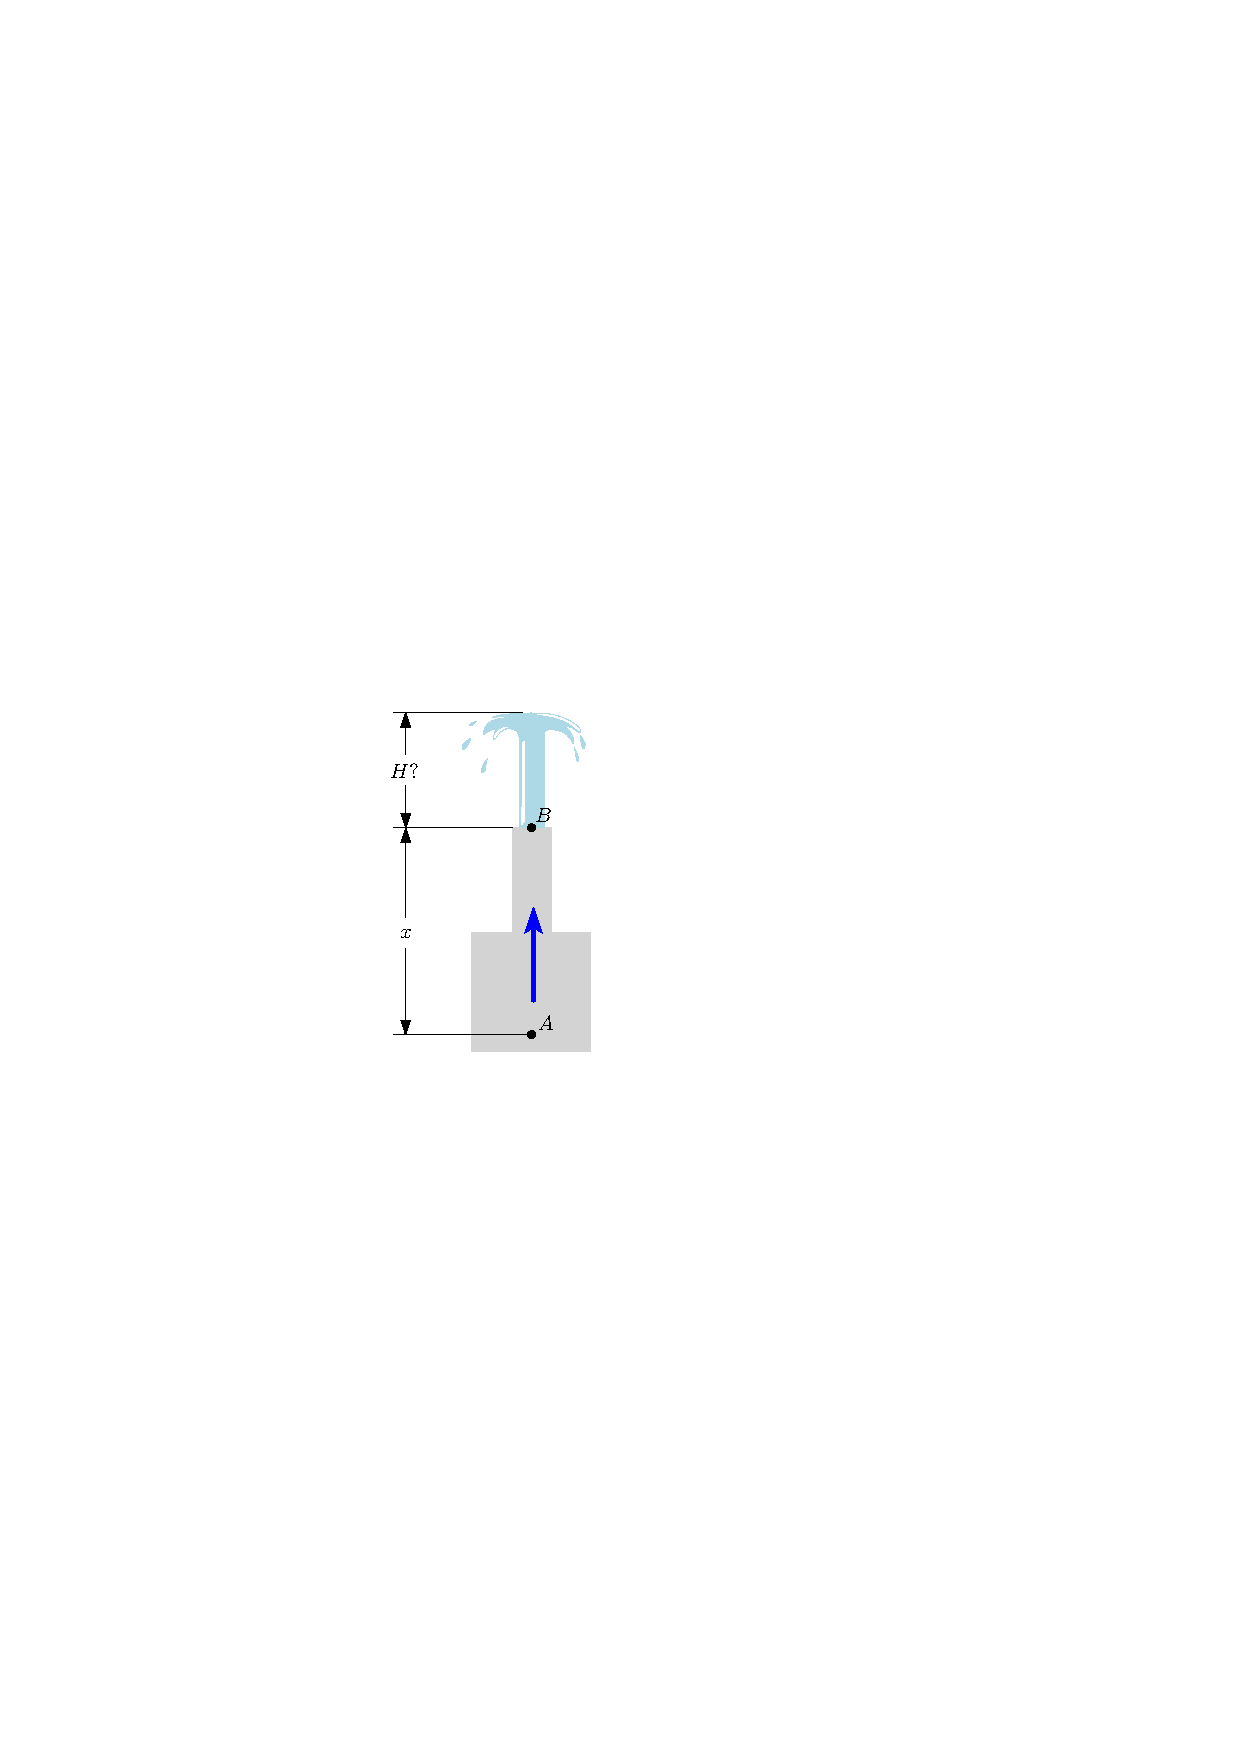
\includegraphics[width=.3\linewidth]{assets/images/ex2}
	\end{center}
	\subsection{Solução}
	O primeiro trecho analisado estabelece a conservação de energia entre as cotas $A$ e $B$. Ao escrever a equação de Bernoulli nesse caso, obtemos
	\begin{equation}
		Z_{A}+\dfrac{v_{A}^{2}}{2g}+\dfrac{p_{A}}{\gamma_{\ce{H2O}}}=Z_{B}+\dfrac{v_{B}^{2}}{2g}+\dfrac{p_{B}}{\gamma_{\ce{H2O}}}+hf_{A-B}
	\end{equation}
	A partir da figura e das considerações feitas no enunciado podemos cancelar os seguintes termos
	\begin{equation}
	\cancel{Z_{A}}+\dfrac{v_{A}^{2}}{2g}+\dfrac{p_{A}}{\gamma_{\ce{H2O}}}=Z_{B}+\dfrac{v_{B}^{2}}{2g}+\cancelto{p_{B}=p_{\text{atm}}}{\dfrac{p_{B}}{\gamma_{\ce{H2O}}}}+\cancel{hf_{A-B}}
	\end{equation}
	logo
	\begin{equation}
	\label{eq:bernoulli2}
	\dfrac{v_{A}^{2}}{2g}+\dfrac{p_{A}}{\gamma_{\ce{H2O}}}=Z_{B}+\dfrac{v_{B}^{2}}{2g}
	\end{equation}
	Como o fluxo que atravessa a seção transversal da tubulação em $A$ e $B$ é o mesmo, é possível determinar a relação entre as velocidades e denotar $v_{B}$ como função de $v_{A}$, assim
	\begin{eqnarray}
		Q_{A}&=&Q_{B}\\
		v_{A}\,A_{A}&=&v_{B}\,A_{B}\\
		v_{A}\,\dfrac{\bcancel{\pi}d_{A}^{2}}{\cancel{4}}&=&v_{B}\,\dfrac{\bcancel{\pi} d_{A}^{2}}{\cancel{4}}\\
		v_{A}\,d_{A}^{2}&=&v_{B}\,d_{B}^{2}
	\end{eqnarray}
	Sendo $d_{A}=4\,d_{B}$, vem
	\begin{eqnarray}
		v_{A}\,(4d_{B})^{2}&=&v_{B}\,d_{B}^{2}\\
		v_{A}&=&\dfrac{v_{B}}{16}
	\end{eqnarray}
	Retornando em \eqref{eq:bernoulli2} e substituindo $v_{A}$
	\begin{eqnarray}
		\dfrac{(v_{B}/16)^{2}}{2g}+\dfrac{p_{A}}{\gamma_{\ce{H2O}}}&=&x+\dfrac{v_{B}^{2}}{2g}\\
		\dfrac{v_{B}^{2}}{512g}+\dfrac{p_{A}}{\gamma_{\ce{H2O}}}&=&x+\dfrac{256\,v_{B}^{2}}{512g}\\
		\dfrac{p_{A}}{\gamma_{\ce{H2O}}}&=&x+\dfrac{255\,v_{B}^{2}}{512g}\\
		\therefore v_{B}^{2}&=&\left(\dfrac{p_{A}}{\gamma_{\ce{H2O}}}-x\right)\dfrac{512g}{255}\label{eq:squaredvb}
	\end{eqnarray}
	Após obter uma relação para $v_{B}$, ao tomar como base as cotas em $B$ e $H$ e aplicar Bernoulli novamente
	\begin{equation}
			Z_{B}+\dfrac{v_{B}^{2}}{2g}+\dfrac{p_{B}}{\gamma_{\ce{H2O}}}=Z_{H}+\dfrac{v_{H}^{2}}{2g}+\dfrac{p_{H}}{\gamma_{\ce{H2O}}}+hf_{B-H}
	\end{equation}
	cancelando os termos pertinentes, temos
	\begin{equation}
		\cancel{Z_{B}}+\dfrac{v_{B}^{2}}{2g}+\cancel{\dfrac{p_{B}}{\gamma_{\ce{H2O}}}}=Z_{H}+\cancel{\dfrac{v_{H}^{2}}{2g}}+\cancel{\dfrac{p_{H}}{\gamma_{\ce{H2O}}}}+\cancel{hf_{B-H}}
	\end{equation}
	então
	\begin{eqnarray}
		\label{eq:bernoulliBtoH}
		\dfrac{v_{B}^{2}}{2g}&=&Z_{H}
	\end{eqnarray}
	Substituindo \eqref{eq:squaredvb} em \eqref{eq:bernoulliBtoH}
	\begin{eqnarray}
		\left(\dfrac{p_{A}}{\gamma_{\ce{H2O}}}-x\right)\dfrac{512\cancel{g}}{255}&=&2\,\cancel{g}\,Z_{H}\\
		Z_{H}&=&\left(\dfrac{p_{A}}{\gamma_{\ce{H2O}}}-x\right)\dfrac{512}{510}\label{eq:zh}
	\end{eqnarray}
	A pressão em $A$ deve ser convertida para Pascal (Pa)
	\begin{eqnarray}
		p_{A}&=&\SI{.58}{\kilogram f/\centi\meter^{2}}\\
			 &=&\dfrac{0.58\cdot 9.81}{(10^{-2})^{2}}\SI{}{\dfrac{\newton}{\meter^{2}}}\\
			 &=&\SI{56898}{\pascal}
	\end{eqnarray}
	e o peso específico em $\SI{}{\newton/\meter^{3}}$
	\begin{eqnarray}
		\gamma_{\ce{H2O}}&=&\SI{1000}{\kilogram f/\meter^{3}}\\
						 &=&1000\cdot 9.81\,\SI{}{\newton/\meter^{3}}\\
						 &=&\SI{9810}{\newton/\meter^{3}}
	\end{eqnarray}
	como $x=\SI{.3}{\meter}$, após substituir em \eqref{eq:zh} é obtido $Z_{H}=H$
	\begin{eqnarray}
		Z_{H}&=&\left(\dfrac{56\,898}{9\,810}-0.3\right)\dfrac{512}{510}\\
			 &=&\purple{\SI{5.52}{\meter}}
	\end{eqnarray}
	\section{Terceira questão}
	A seção 1 possui diâmetro de \SI{15.4}{\milli\meter}, pressão manométrica de \SI{331}{\kilo\pascal} e velocidade média de escoamento de \SI{2}{\meter/\second}. A seção 2 possui \SI{58.9}{\milli\meter} de diâmetro. Supondo que não existe perdas de energia entre os pontos 1 e 2, calcular a pressão relativa no ponto 2 (resposta em \SI{}{\kilo\pascal}, com 2 casas decimais). Os desníveis verticais em relação ao plano de referência são: $h_{1}=\SI{0}{\meter}$ e $h_{2}=\SI{4.9}{\meter}$. O fluido é água, cujo peso específico é $\SI{9810}{\newton/\meter^{3}}$.
	\begin{center}
		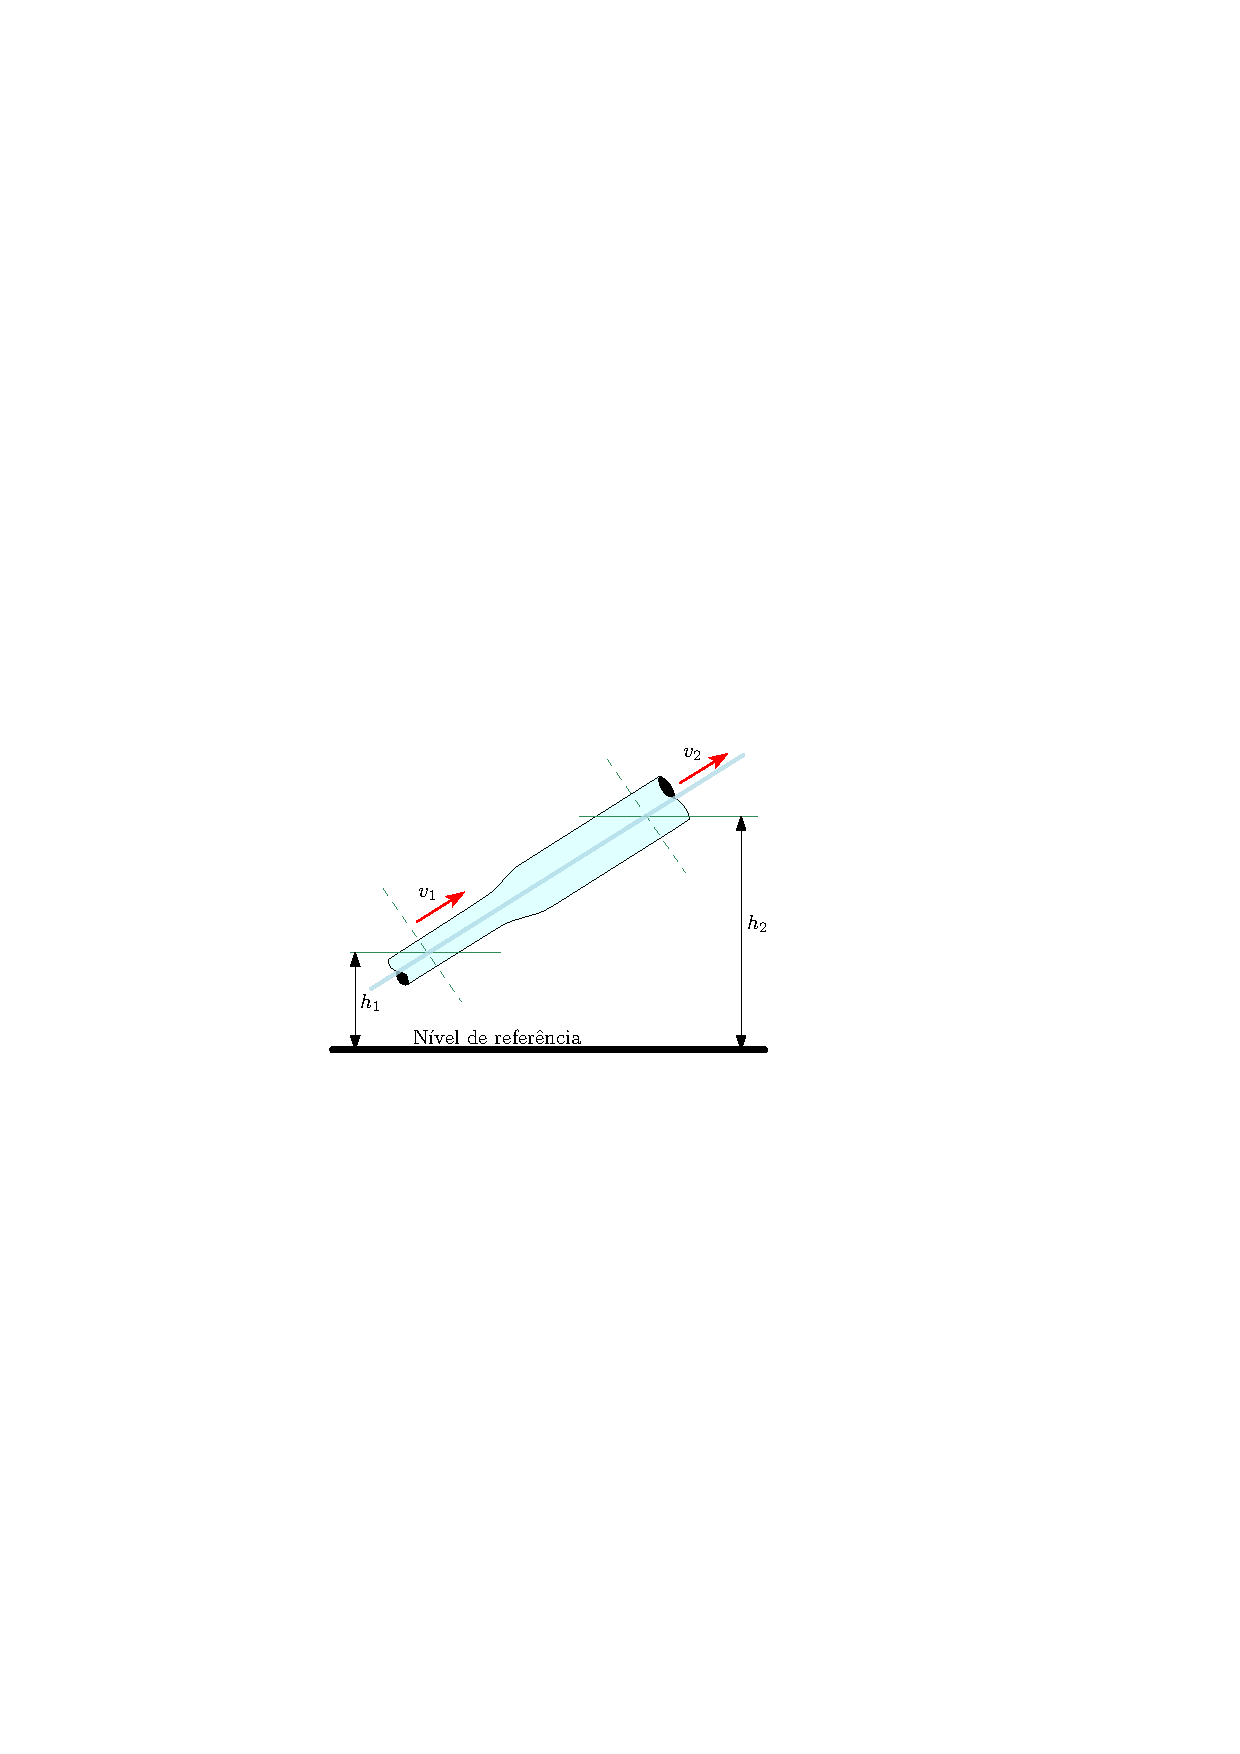
\includegraphics[width=.6\linewidth]{assets/images/ex3}
	\end{center}
	\subsection{Solução}
	A vazão no tubo é constante, logo
	\begin{eqnarray}
		Q_{1}&=&Q_{2}\\
		v_{1}\,A_{1}&=&v_{2}\,A_{2}\\
		v_{1}\,d_{1}^{2}&=&v_{2}\,d_{2}^{2}\\
		v_{2}&=&\dfrac{v_{1}\,d_{1}^{2}}{d_{2}^{2}}
	\end{eqnarray}
	Substituindo, vem
	\begin{eqnarray}
		v_{2}&=&\dfrac{2\cdot 0.0154^{2}}{0.0589^{2}}\\
			 &=&\SI{.1367}{\meter/\second}
	\end{eqnarray}
	Com a velocidade do fluído no ponto 2 calculada, se aplicarmos Bernoulli des\-prezando a cota em 1, chegamos que
	\begin{eqnarray}
		\cancel{Z_{1}}+\dfrac{v_{1}^{2}}{2g}+\dfrac{p_{1}}{\gamma_{\ce{H2O}}}&=&Z_{2}+\dfrac{v_{2}^{2}}{2g}+\dfrac{p_{2}}{\gamma_{\ce{H2O}}}+\cancelto{\textrm{desprezível}}{hf_{1-2}}\\
		p_{2}&=&\gamma_{\ce{H2O}}\left(\dfrac{v_{1}^{2}-v_{2}^{2}}{2g}+\dfrac{p_{1}}{\gamma_{\ce{H2O}}}-Z_{2}\right)\\
			 &=&9\,810\cdot\left(\dfrac{2^{2}-0.1367^{2}}{2\cdot 9.81}+\dfrac{331\,000}{9\,810}-4.9\right)\\
			 &=&\SI{284921.653}{\pascal}=\purple{\SI{284.92}{\kilo\pascal}}
	\end{eqnarray}
	\section{Quarta questão}
	Na figura, os diâmetros da sucção e recalque são de 3 e 2 polegadas, respectivamente. As pressões relativas nos pontos 1 e 2 são \SI{-12.9}{\kilo\pascal} e \SI{336.8}{\kilo\pascal}, respectivamente. Pela tubulação passa água na vazão de \SI{1093}{\liter/\minute}. A perda de carga entre os pontos 1 e 2 é de \SI{1.25}{\meter} e o desnível vertical $h$ é de \SI{9.1}{\meter}. Calcule a potência hidráulica da bomba em cv (uma casa decimal).
	\begin{center}
		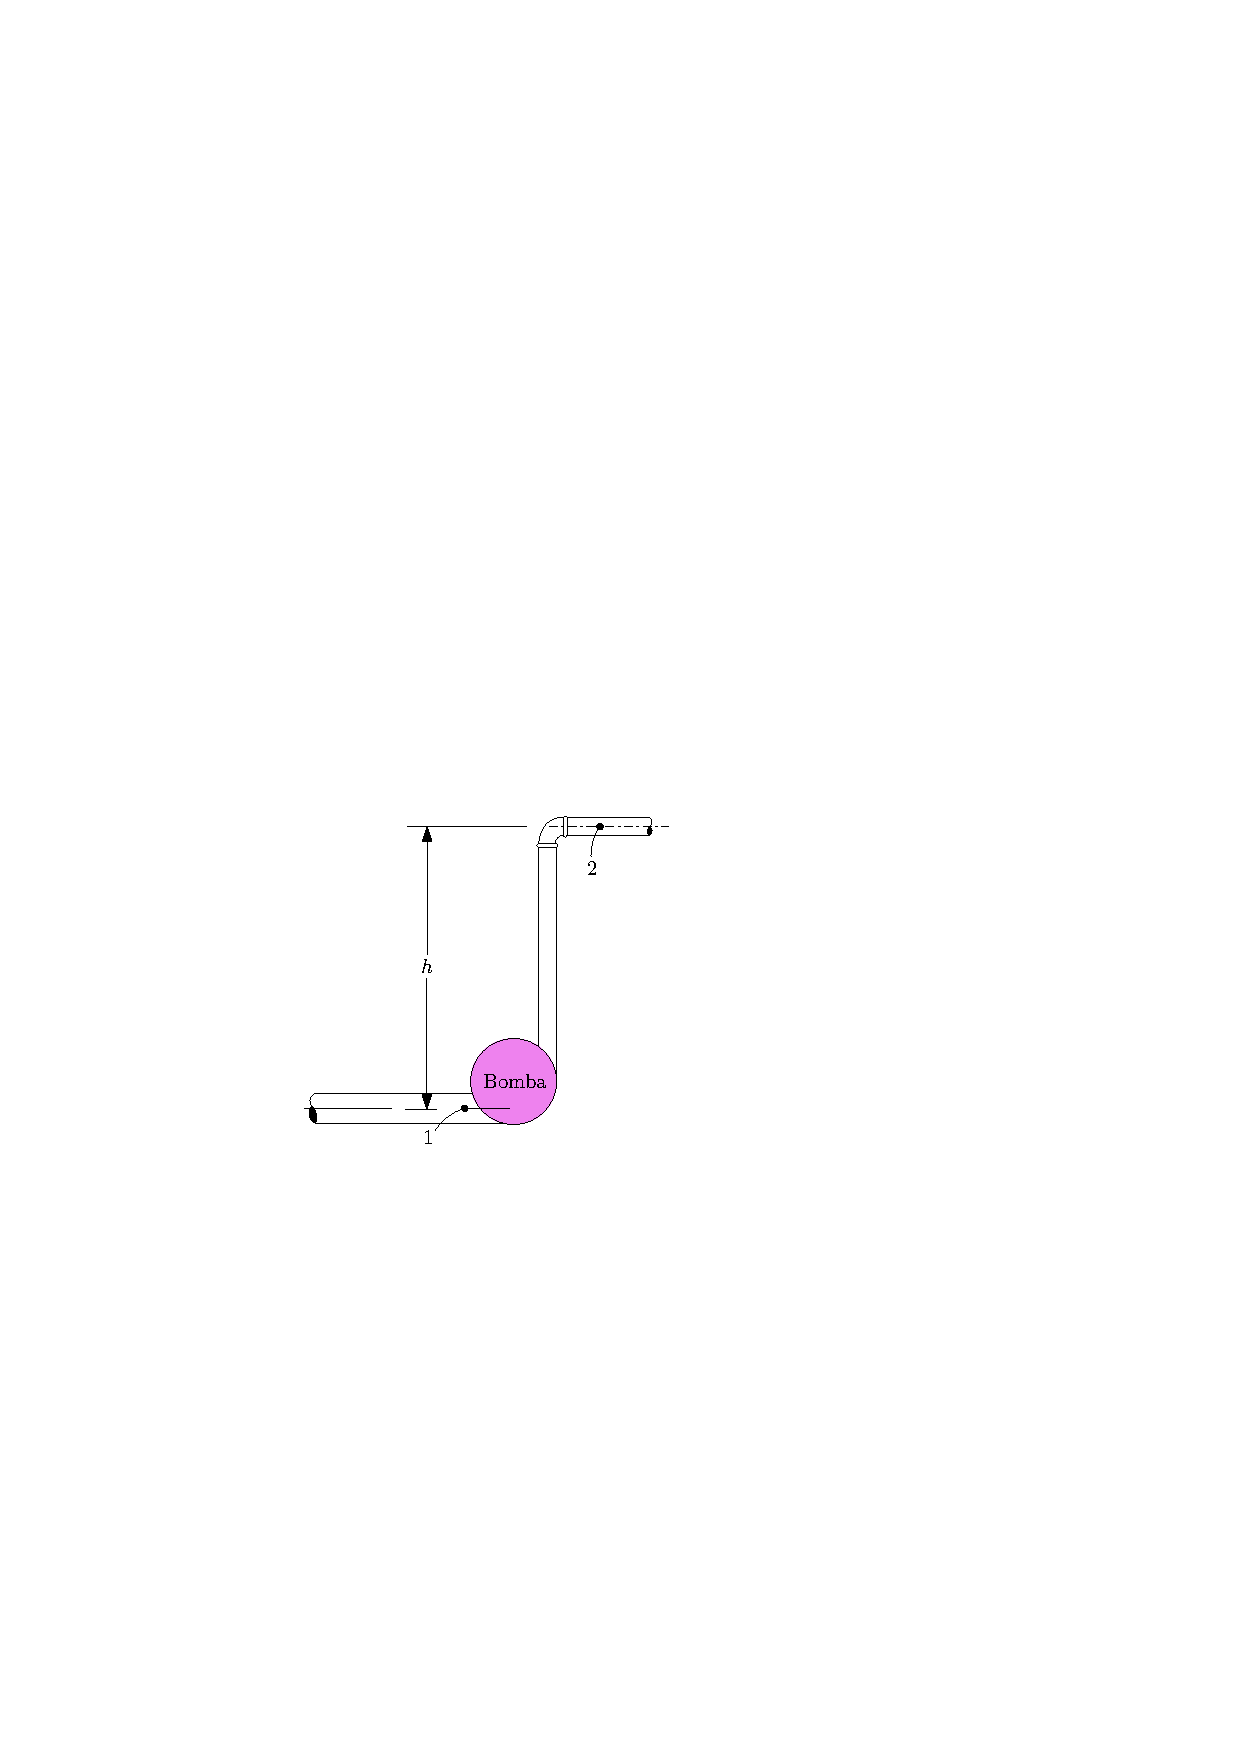
\includegraphics[width=.55\linewidth]{assets/images/ex4}
	\end{center}
	\begin{itemize}
		\item $\SI{735}{\watt}=\SI{1}{cv}$
		\item $\gamma_{\ce{H2O}}=\SI{9810}{\newton/\meter^{3}}$
		\item Água escoa de 1 para 2.
		\item Desprezar variação de carga cinética. entre os pontos 1 e 2.
	\end{itemize}
	\subsection{Solução}
	Inicialmente é necessário converter a vazão dada em litros por minuto (\SI{}{\liter/\minute}) para metros cúbicos por segundo ($\SI{}{\meter^{3}/\second}$), assim
	\begin{eqnarray}
		Q&=&\SI{1093}{\liter/\minute}\\
		 &=&\dfrac{1093\cdot 10^{-3}}{60}\SI{}{\dfrac{\meter^{3}}{\second}}\\
		 &=&\SI{1.821667e-2}{\meter^{3}/\second}
	\end{eqnarray}
	Aplicando Bernoulli contabilizando o efeito da bomba do lado esquerdo da equação, obtemos
	\begin{equation}
		Z_{1}+\dfrac{v_{1}^{2}}{2g}+\dfrac{p_{1}}{\gamma_{\ce{H2O}}}+h_{b}=Z_{2}+\dfrac{v_{2}^{2}}{2g}+\dfrac{p_{2}}{\gamma_{\ce{H2O}}}+hf_{1-2}\\
	\end{equation}
	Ao desprezar a cota no ponto 1, os dois termos de carga cinética em cada lado da equação anterior e isolar $h_{b}$, temos
	\begin{equation}
		h_{b}=\dfrac{p_{2}-p_{1}}{\gamma_{\ce{H2O}}}+Z_{2}+hf_{1-2}
	\end{equation}
	Após multiplicar por 1000 as pressões em \SI{}{\kilo\pascal} e desenvolver os cálculos
	\begin{eqnarray}
		h_{b}&=&\dfrac{336\,800-(-12\,900)}{9810}+9.1+1.25\\
			 &\approx&\SI{46}{\meter}
	\end{eqnarray}
	Dessa forma, a potência dissipada pela bomba é dada por
	\begin{equation}
		P=\gamma_{\ce{H2O}}\,Q\,h_{b}
	\end{equation}
	Substituindo
	\begin{eqnarray}
		P&=&9810\cdot 1.821667\cdot 10^{-2}\cdot 46\\
		 &=&\SI{8220.454}{\watt}=\purple{\SI{11.2}{cv}}
	\end{eqnarray}
	\section{Quinta questão}
	A figura abaixo representa um Tubo Venturi empregado para a medição de vazão em condutos pressurizados. O Tubo Venturi está equipado com um manômetro diferencial de mercúrio. O diâmetro da seção de escoamento 1 é \SI{14.5}{\centi\meter} e da seção 2 é \SI{3.3}{\centi\meter}. Calcular a vazão teórica de água sabendo que a deflexão manométrica $\Delta h$ é \SI{34.3}{\centi\meter}. Expressar a resposta em $\SI{}{\meter^{3}/\hour}$ com duas casas decimais.
	\begin{center}
		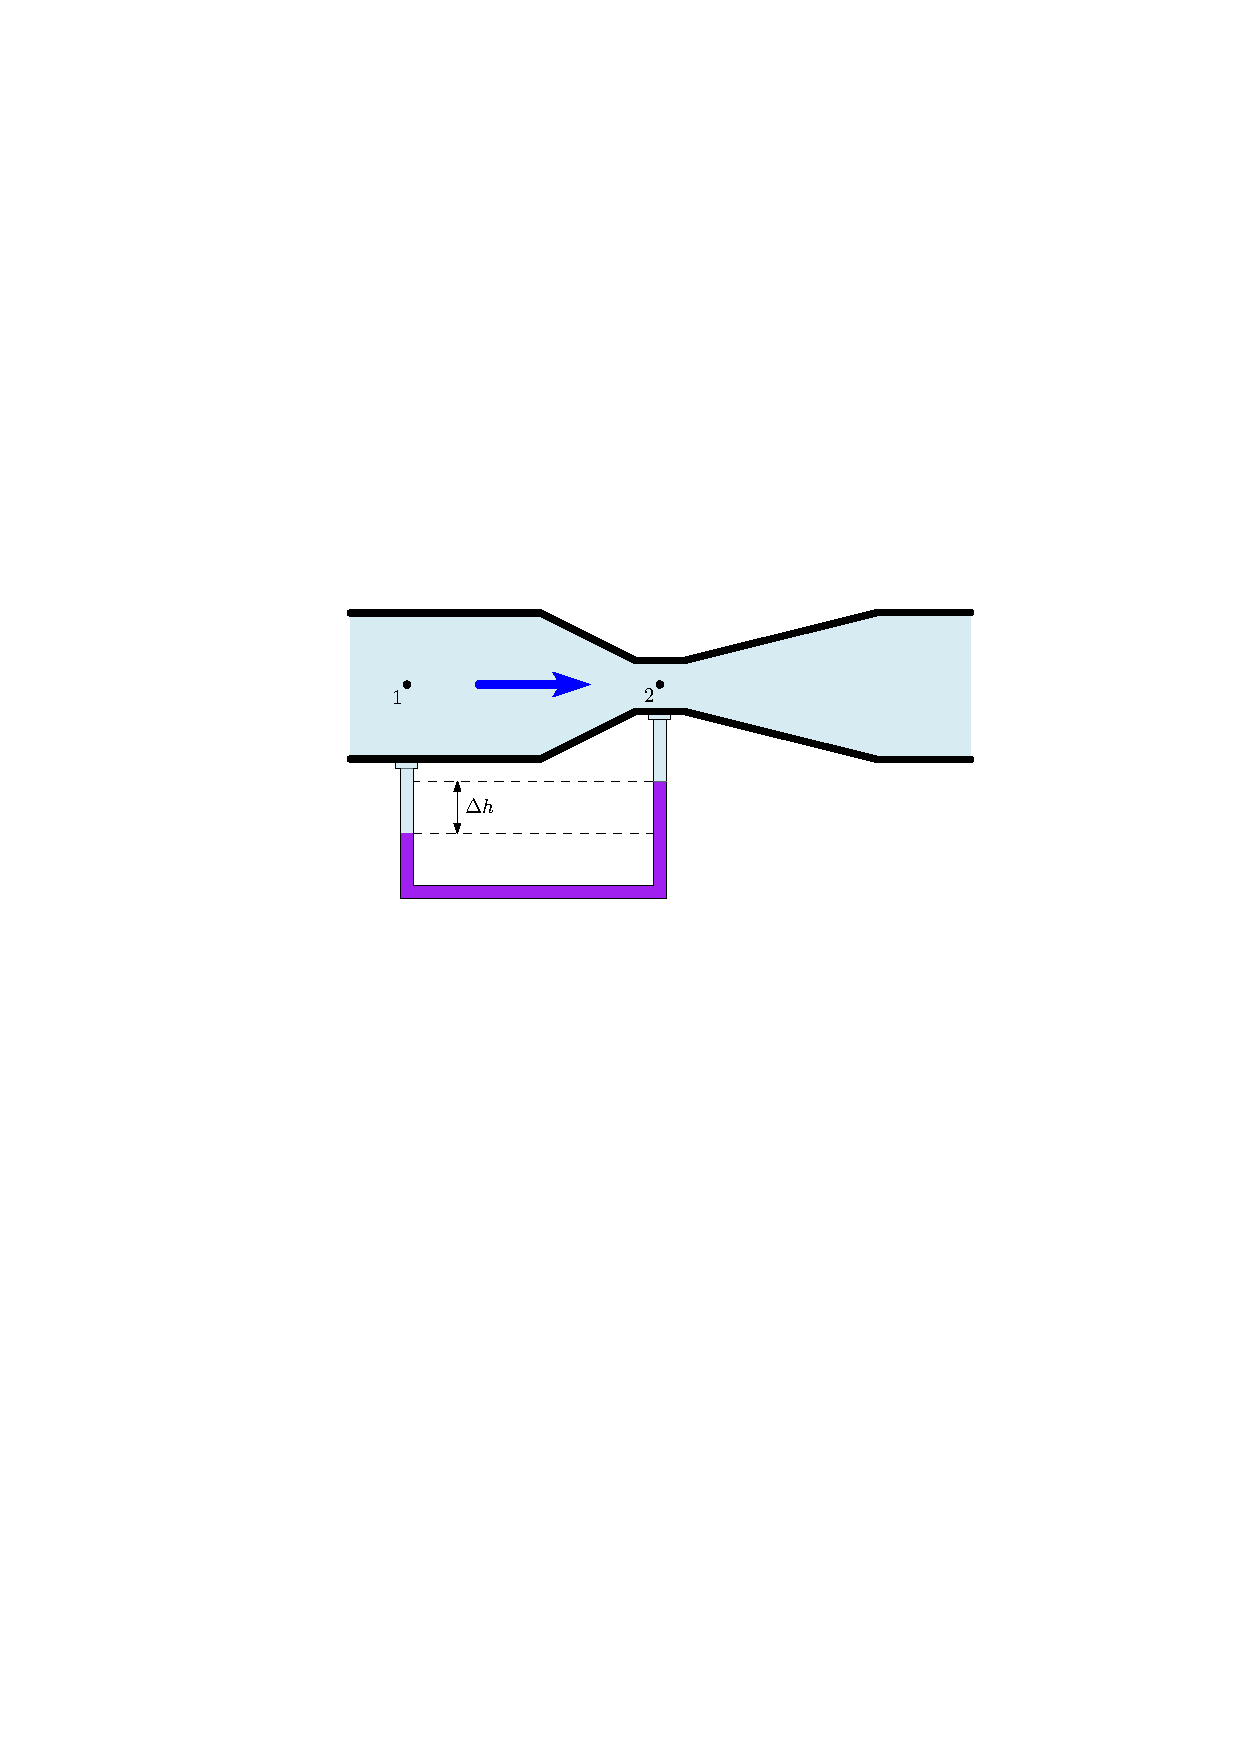
\includegraphics[width=.9\linewidth]{assets/images/ex5}
	\end{center}
	\noindent Informações adicionais:
	\begin{itemize}
		\item Tubo de Venturi está instalado em nível.
		\item Despreza a perda de carga entre os ponto. 1 e 2 
		\item $\rho_{\ce{Hg}}=\SI{13.6}{\gram/\centi\meter^{3}}$
		\item $\rho_{\ce{H2O}}=\SI{1000}{\kilogram/\meter^{3}}$
	\end{itemize}
	\subsection{Solução}
	Primeiramente, estabelecendo o referencial na parte inferior do tubo é possível obter a relação das pressões atuantes em cada ponto devido a ação das colunas de água e mercúrio acima de cada um e, a partir disso, chegar numa equação que relaciona a diferença de pressão entre os pontos 1 e 2, como segue
	\begin{center}
		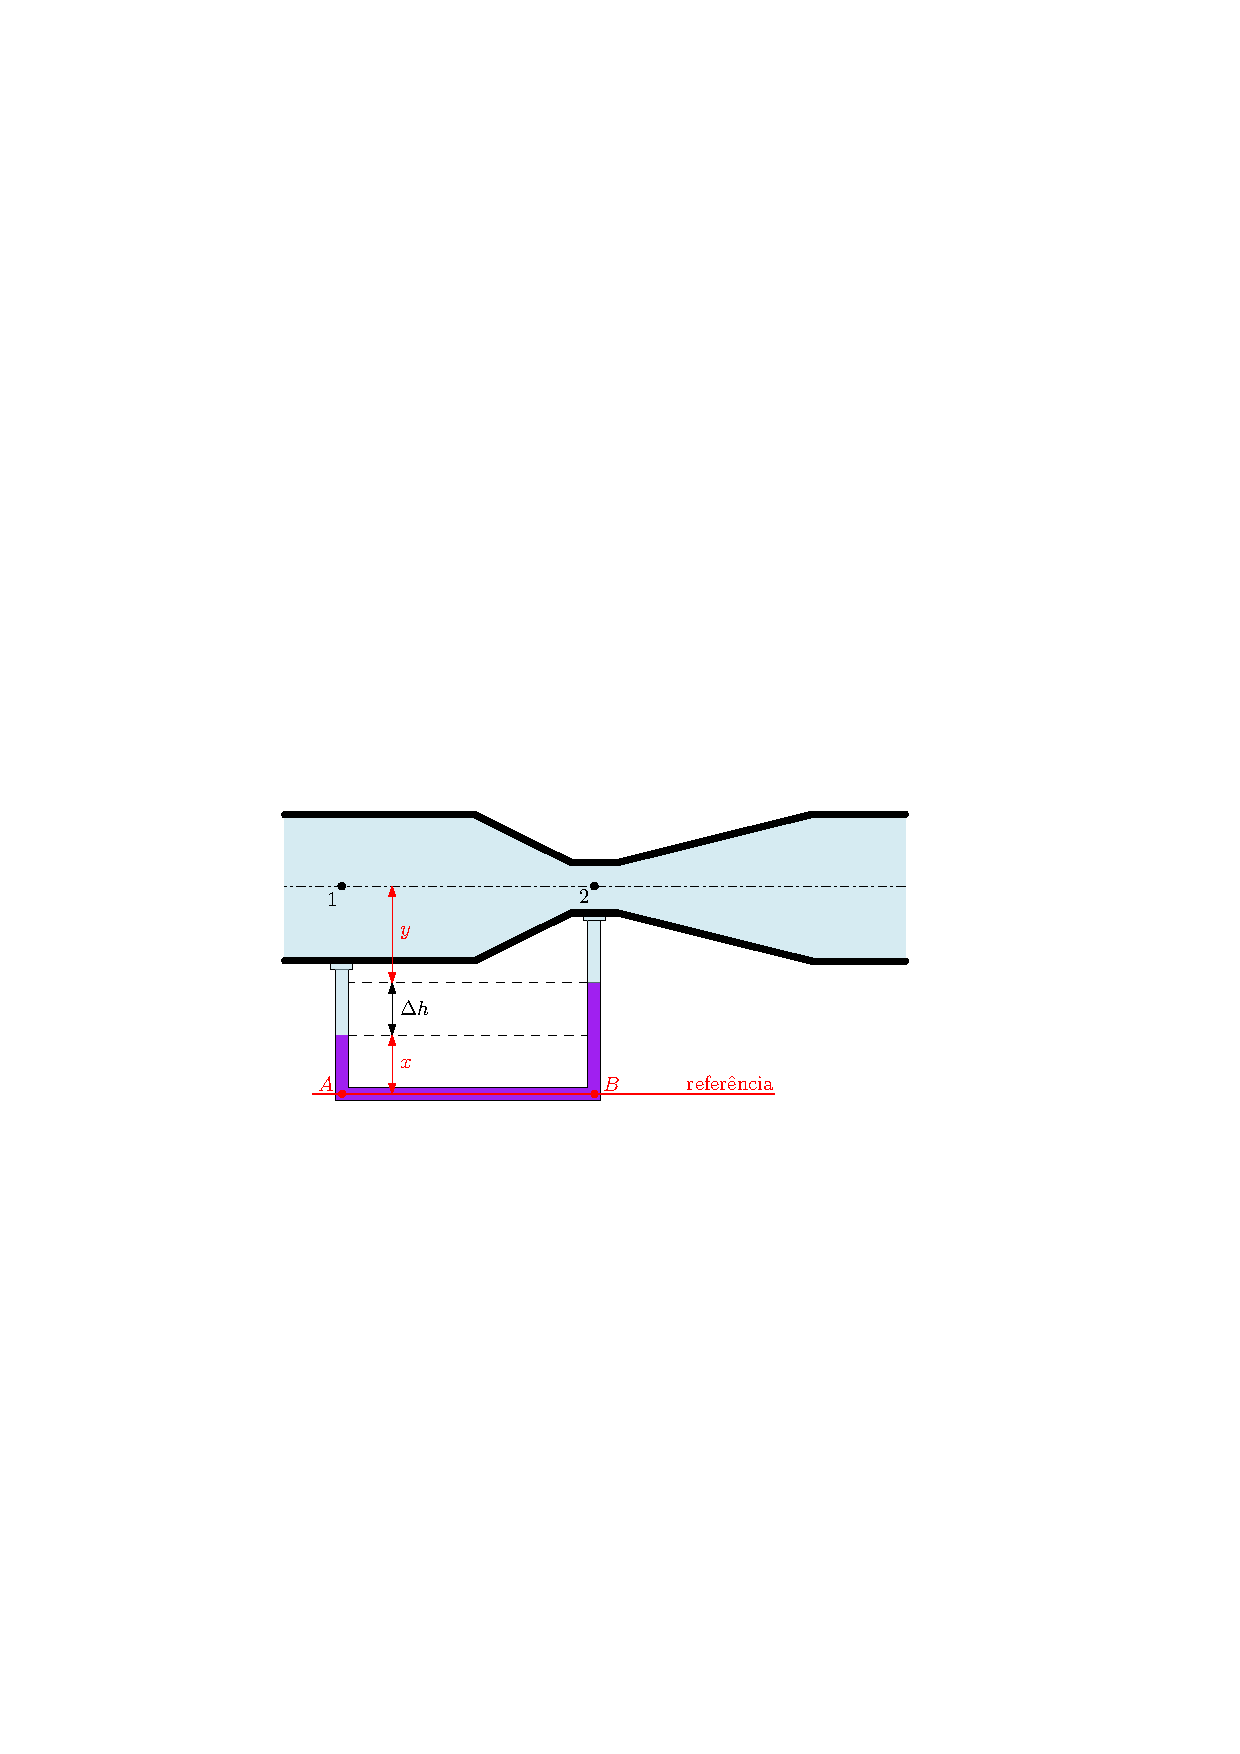
\includegraphics[width=.9\linewidth]{assets/images/referencia_5}
	\end{center}

	$$
	\begin{cases}
		p_{A}=\gamma_{\ce{H2O}}(y+\Delta h)+\gamma_{\ce{Hg}}\,x+p_{1}\\
		p_{B}=\gamma_{\ce{H2O}}\,y+\gamma_{\ce{Hg}}(\Delta h+x)+p_{2}
	\end{cases}
	\Rightarrow
	\begin{cases}
		p_{A}=\gamma_{\ce{H2O}}\,y+\gamma_{\ce{H2O}}\,\Delta h+\gamma_{\ce{Hg}}\,x+p_{1}\\
		p_{B}=\gamma_{\ce{H2O}}\,y+\gamma_{\ce{Hg}}\,\Delta h+\gamma_{\ce{Hg}}\,x+p_{2}
	\end{cases}
	$$
	Como $p_{A}=p_{B}$
	\begin{eqnarray}
		\gamma_{\ce{H2O}}\,y+\gamma_{\ce{H2O}}\,\Delta h+\gamma_{\ce{Hg}}\,x+p_{1}&=&\gamma_{\ce{H2O}}\,y+\gamma_{\ce{Hg}}\,\Delta h+\gamma_{\ce{Hg}}\,x+p_{2}\\
		\cancel{\gamma_{\ce{H2O}}\,y}+\gamma_{\ce{H2O}}\,\Delta h+\bcancel{\gamma_{\ce{Hg}}\,x}+p_{1}&=&\cancel{\gamma_{\ce{H2O}}\,y}+\gamma_{\ce{Hg}}\,\Delta h+\bcancel{\gamma_{\ce{Hg}}\,x}+p_{2}
	\end{eqnarray}
	Isolando a diferença $p_{1}-p_{2}$
	\begin{equation}
		\label{eq:ps}
		p_{1}-p_{2}=(\gamma_{\ce{Hg}}-\gamma_{\ce{H2O}})\,\Delta h
	\end{equation}
	Feito isso, se analisarmos o Tubo de Venturi nos pontos 1 e 2 a aplicarmos Bernoulli, vem
	\begin{equation}
		Z_{1}+\dfrac{v_{1}^{2}}{2g}+\dfrac{p_{1}}{\gamma_{\ce{H2O}}}=Z_{2}+\dfrac{v_{2}^{2}}{2g}+\dfrac{p_{2}}{\gamma_{\ce{H2O}}}+hf_{1-2}
	\end{equation}
	Como o tubo está em nível as cargas de posição podem ser desprezadas. O mesmo vale para o último termo do lado direito da equação que corresponde à perda de carga de 1 para 2. 
	\begin{equation}
		\cancel{Z_{1}}+\dfrac{v_{1}^{2}}{2g}+\dfrac{p_{1}}{\gamma_{\ce{H2O}}}=\cancel{Z_{2}}+\dfrac{v_{2}^{2}}{2g}+\dfrac{p_{2}}{\gamma_{\ce{H2O}}}+\bcancel{hf_{1-2}}
	\end{equation}
	Portanto
	\begin{equation}
		\label{eq:vel}
		\dfrac{v_{1}^{2}}{2g}+\dfrac{p_{1}}{\gamma_{\ce{H2O}}}=\dfrac{v_{2}^{2}}{2g}+\dfrac{p_{2}}{\gamma_{\ce{H2O}}}
	\end{equation}
	Após obter a equação anterior que relaciona as velocidades e as pressões da água em cada ponto, é necessário encontrar outra relação entre as velocidades que permita que a equação de cima dependa de apenas uma delas. Sabe-se que o fluxo que atravessa 1 e 2 é o mesmo, sendo assim aplicando a equação da continuidade podemos escrever
	\begin{equation}
		v_{1}\,d_{1}^{2}=v_{2}\,d_{2}^{2}
	\end{equation}
	Ao substituir os valores de diâmetros fornecidos, temos
	\begin{eqnarray}
		v_{1}\cdot 0.145^{2}&=&v_{2}\cdot 0.033^{2}\\
		\therefore v_{2}&\approx&19.3067\cdot v_{1}\label{eq:v2}
	\end{eqnarray}
	Substituindo \eqref{eq:v2} em \eqref{eq:vel} e manipulando a equação
	\begin{equation}
		\label{eq:v1}
		v_{1}=\sqrt{\dfrac{g\,(p_{1}-p_{2})}{185.8744\cdot\gamma_{\ce{H2O}}}}
	\end{equation}
	Retornando em \eqref{eq:ps} e substituindo os pesos específicos e a deflexão manométrica fornecidos, vem
	\begin{eqnarray}
		p_{1}-p_{2}&=&(13\,600-1000)\cdot 9.81\cdot 0.343\\
				   &=&\SI{42396.858}{\pascal}
	\end{eqnarray}
	Ao substituir o valor obtido anteriormente em \eqref{eq:v1}, chegamos que
	\begin{eqnarray}
		v_{1}&=&\sqrt{\dfrac{9.81\cdot 42\,396.858}{185.8744\cdot 9810}}\\
		 	 &=&\SI{0.4776}{\meter/\second}
	\end{eqnarray}
	Logo o fluxo no tubo será
	\begin{eqnarray}
		Q&=&Q_{1}\\
		 &=&v_{1}\cdot A_{1}\\
		 &=&v_{1}\cdot\dfrac{\pi d_{1}^{2}}{4}\\
		 &=&0.4776\cdot\dfrac{\pi\cdot 0.145^{2}}{4}\\
		 &=&\SI{7.886607e-3}{\meter^{3}/\second}=\purple{\SI{28.39}{\meter^{3}/\hour}}
	\end{eqnarray}
\end{document}